
\documentclass[ms.tex]{subfiles}
\begin{document}

\section{Mock Samples}
\label{sec:mocks}

Using our parametrization of one-zone GCE models described
in~\S~\ref{sec:onezone}, here we define a set of parameter choices from which
mock samples of stars can be drawn.
We then demonstrate the validity of our likelihood function (equation
\ref{eq:likelihood}) in~\S~\ref{sec:mocks:recovered} by applying it to a
fiducial mock sample and comparing the best-fit values to the known parameters
of the input model.
In~\S~\ref{sec:mocks:variations}, we then explore variations in sample size,
measurement precision, and the availability of age information.

\subsection{A Fiducial Mock Sample}
\label{sec:mocks:fiducial}

% fig 1
\begin{figure*}
\centering
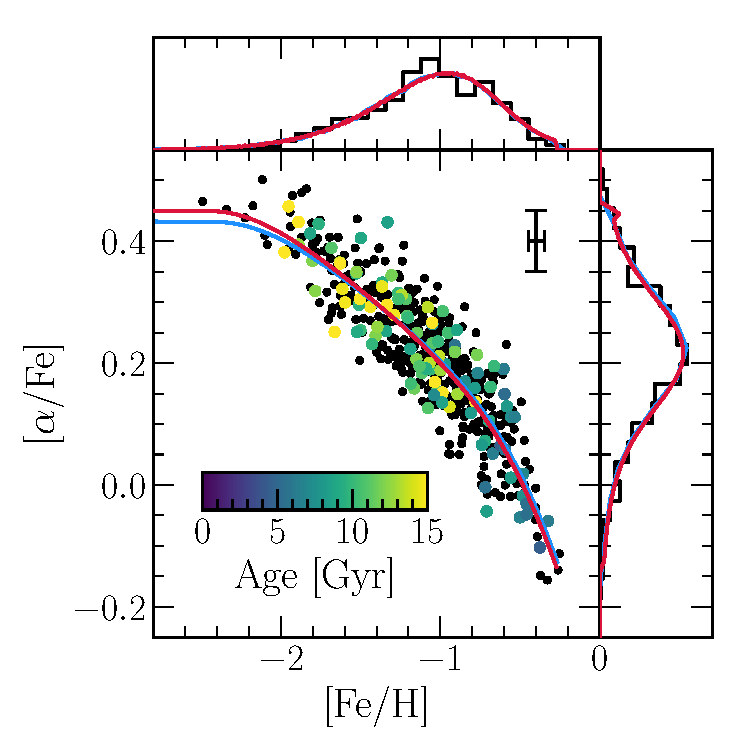
\includegraphics[scale = 0.5]{fiducial_mock_afe_feh.pdf}
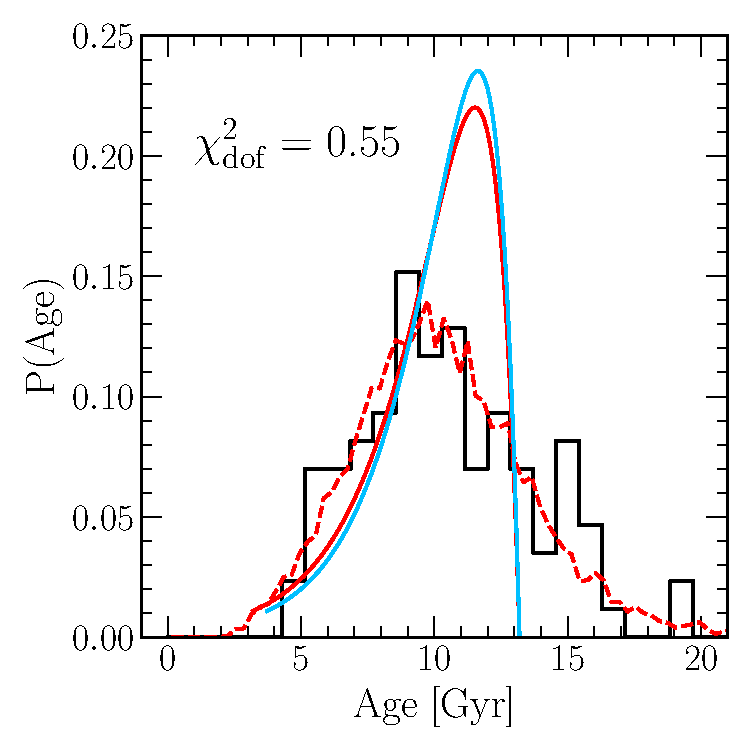
\includegraphics[scale = 0.42]{fiducial_mock_agedist.pdf}
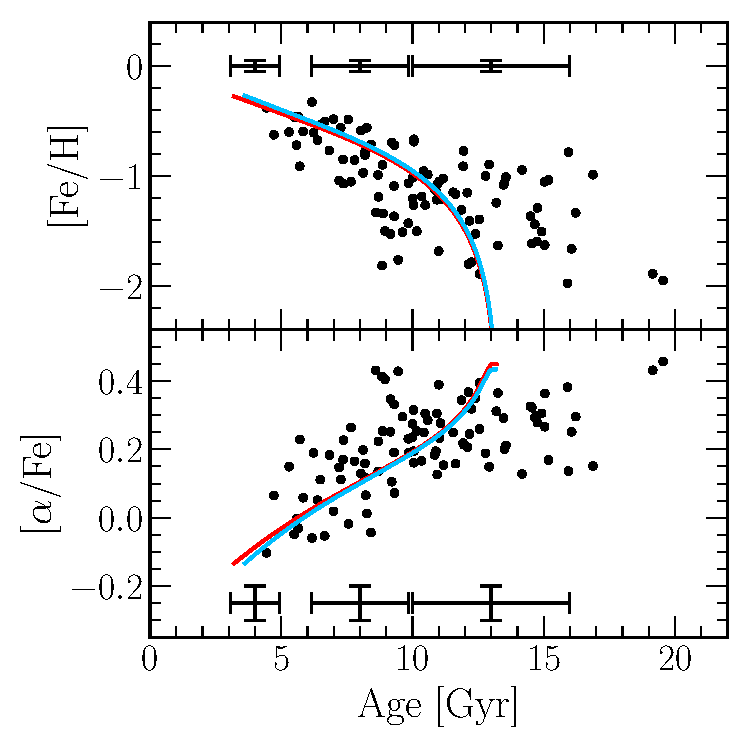
\includegraphics[scale = 0.42]{fiducial_mock_amr.pdf}
\caption{
\textbf{Left}: Our fiducial mock sample in the~\afe-\feh~plane.
There are~$N = 500$ stars with abundance uncertainties of~$\sigma_\feh =
\sigma_\afe = 0.05$ as indicated by the errorbar.
$N = 100$ of the stars have age information as indicated by the colorbar with
an artificial uncertainty of~$\sigma_{\log_{10}(\text{age})} = 0.1$.
On the top and right, we show the marginalized distributions in~\afe~and~\feh,
with red lines denoting the known distribution.
\textbf{Center}: The age distribution of the mock sample (black, binned).
The dashed red line indicates the age distribution that is obtained by sampling
$N = 10^4$ rather than~$N = 500$ stars from the input model and assuming the
same age uncertainty.
\textbf{Right}: The age-\feh~(top) and age-\afe~(bottom) relations for the
mock sample with artificial uncertainties denoted by the error bars on each
panel.
Solid red and blue lines in all panels denote the known relations from the
input model and the recovered best-fit model, respectively.
}
\label{fig:fiducial_mock}
\end{figure*}

% fig 2
\begin{figure*}
\centering
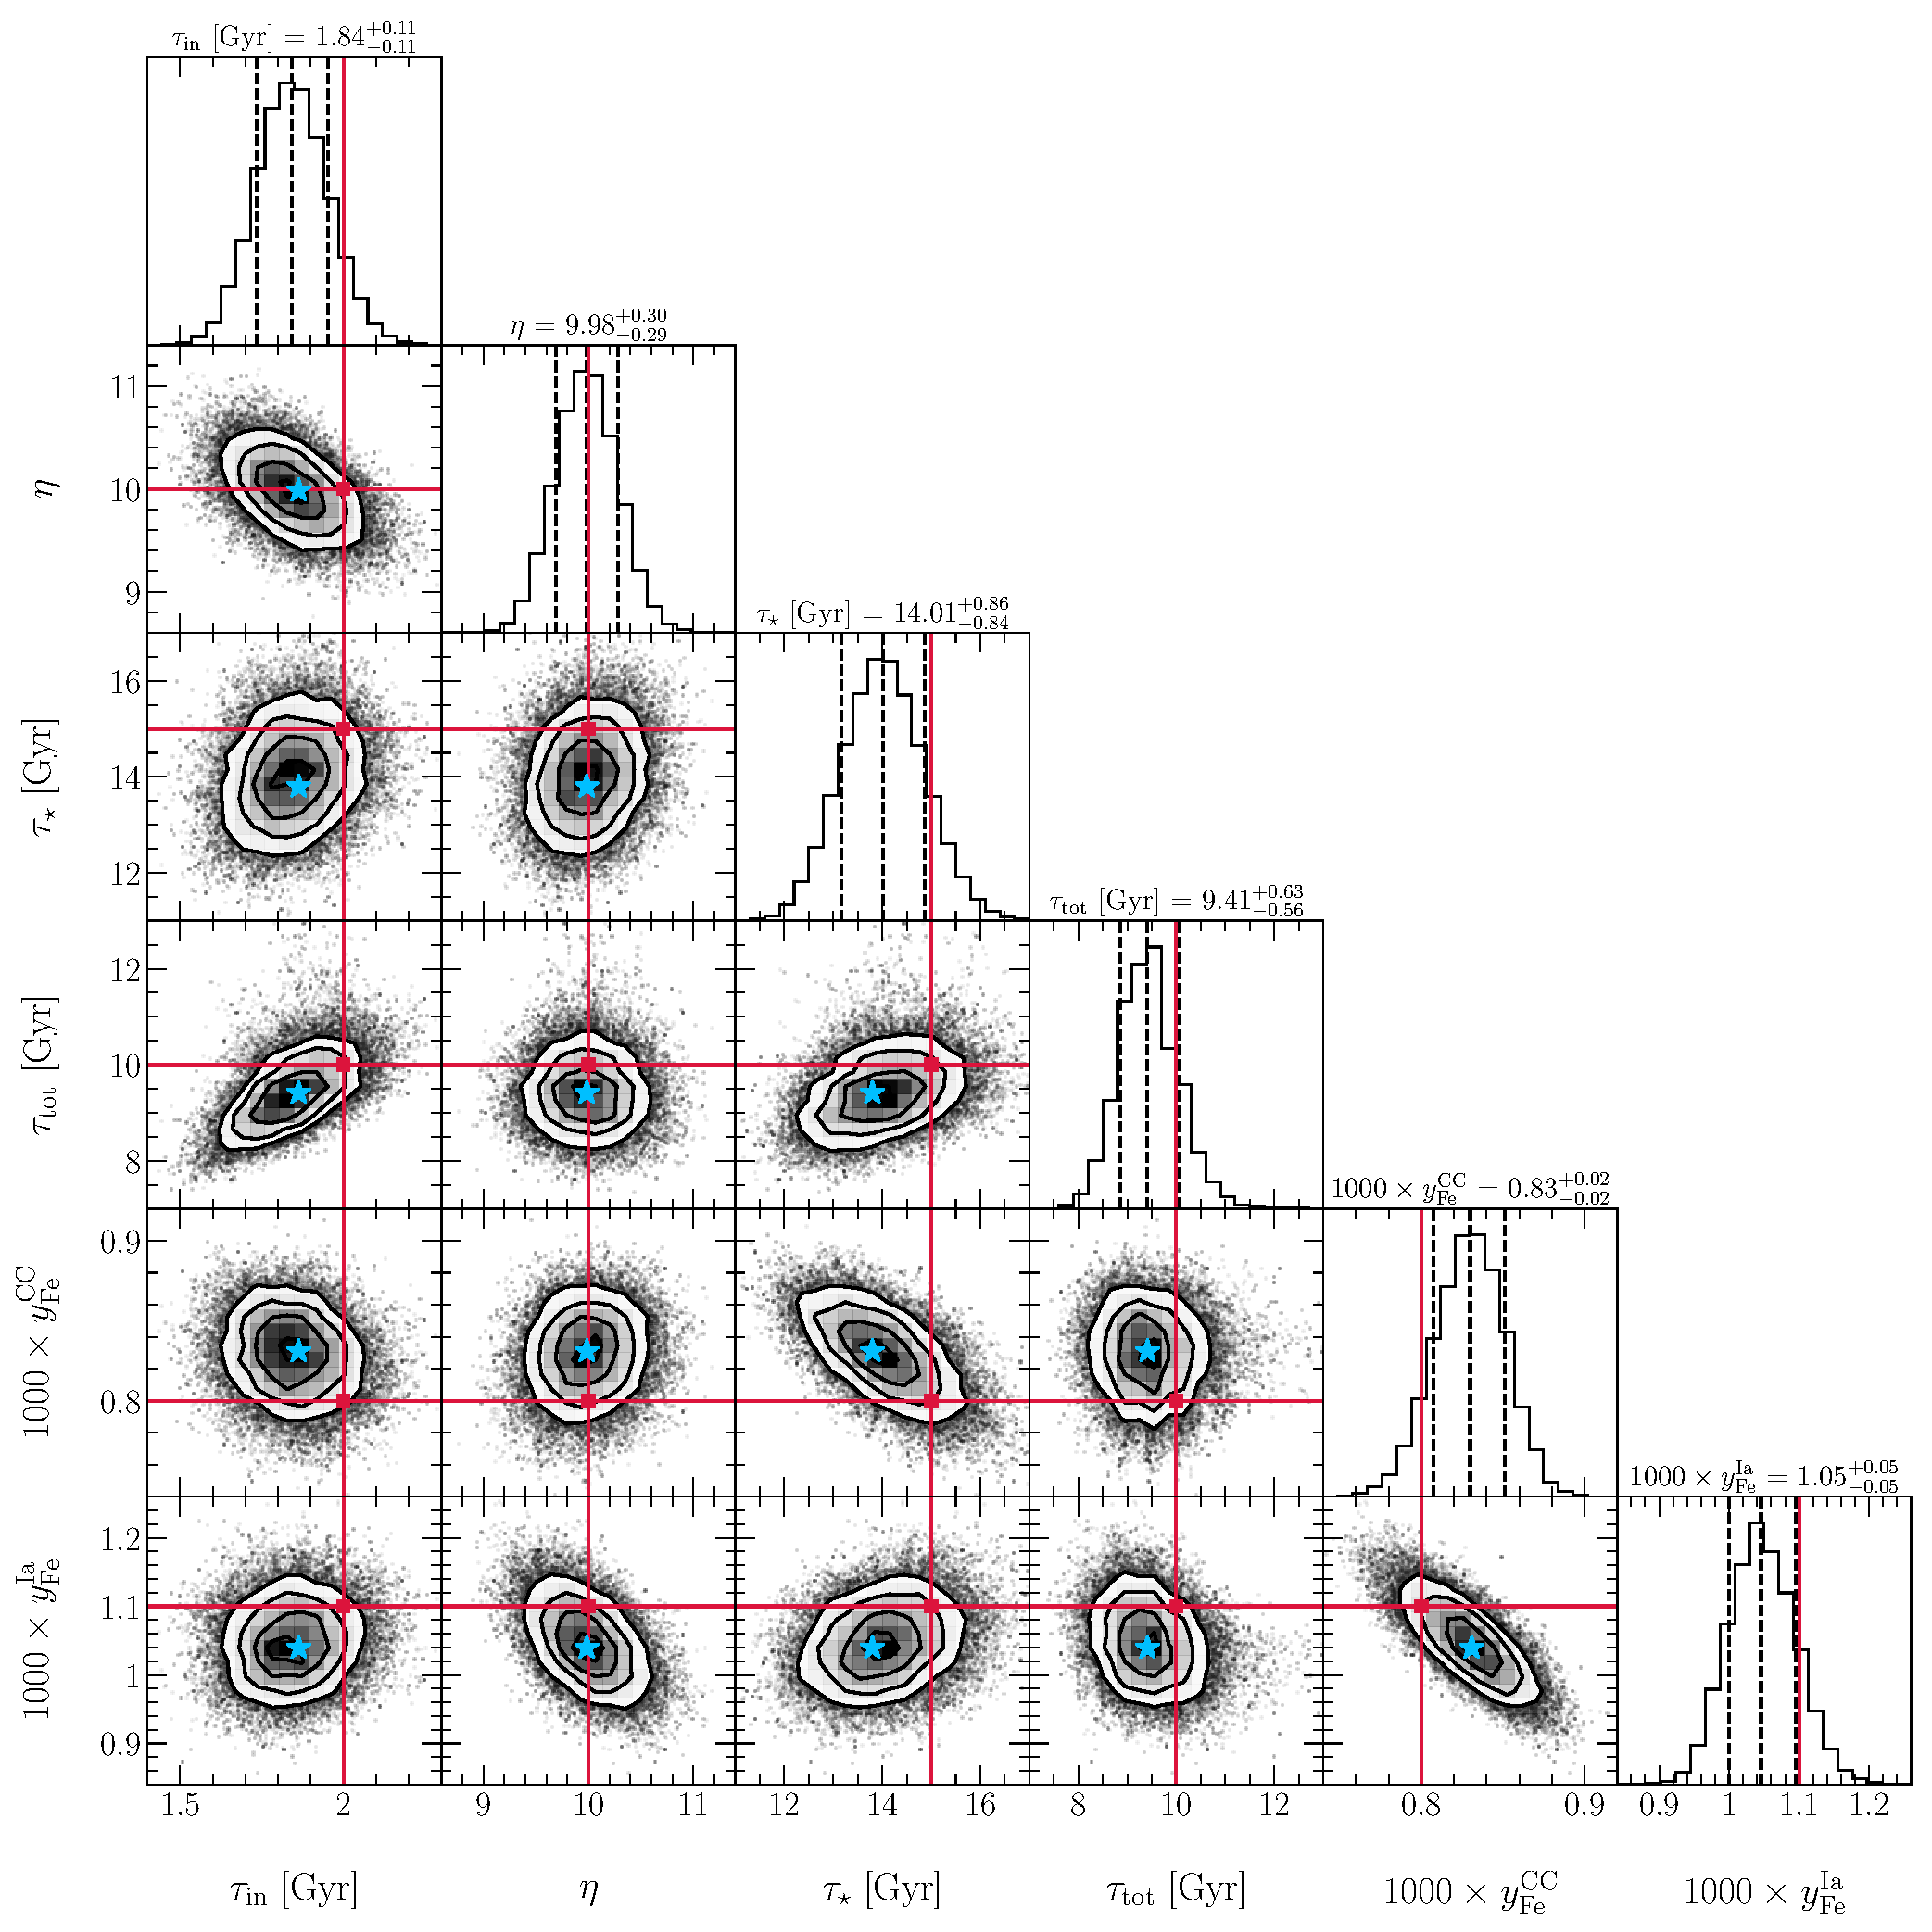
\includegraphics[scale = 0.5]{fiducial_76k8.pdf}
\caption{
The ``corner-plot'' showing the results of applying our fitting method to our
fiducial mock sample (see discussion in~\S\S~\ref{sec:fitting} and
\ref{sec:mocks:fiducial}).
Panels along the diagonal show the marginalized likelihood distribution in each
parameter along with their best-fit values and confidence intervals.
Panels below the diagonal show 2-dimensional cross-sections of the
6-dimensional likelihood function.
Blue stars mark the element of the Markov chain with the maximum likelihood.
Red ``cross-hairs'' denote the true, nown values of the parameters from the
input model (see the top row of Table X).
}
\label{fig:fiducial_mock_corner}
\end{figure*}

We take an exponential infall history~$\dot{M}_\text{in} \propto e^{-t /
\tau_\text{in}}$ with an e-folding timescale of~$\tau_\text{in} = 2$ Gyr and an
initial ISM mass of~$M_\text{g} = 0$.
We select an SFE timescale of~$\tau_\star = 15$ Gyr, motivated by the
observational result that dwarf galaxies have generally inefficient star
formation~\citep[e.g.][]{Hudson2015}.
We additionally select a mass-loading factor of~$\eta = 10$ because the
strength of outflows should, in principle, contain information on the depth of
the gravity well of a given galaxy, with lower mass systems being more
efficient at ejecting material from the ISM.
If the SFH in this model were constant, the analytic formulae of
\citet{Weinberg2017} suggest that the equilibrium alpha element abundance
should be~$\sim16$\% of the solar oxygen abundance, in qualitative agreement
with the empirical mass-metallicity relation for galaxies
(\citealp{Tremonti2004, Gallazzi2005};~\citealp*{Zahid2011};
\citealp{Andrews2013, Kirby2013, Zahid2014}).
\par
With these choices regarding~$\tau_\star$ and~$\eta$, our parameters are in
the regime where the normalization of the infall history, and consequently the
SFH, is inconsequential to the predicted evolution of the abundances.
The appropriate likelihood function is therefore equation~\refp{eq:likelihood}
with normalized weights, whereas equation~\refp{eq:lnL_minus_weights} with
un-normalized weights would be the proper form if we had selected a
parametrization in which the absolute scale of the SFH impacts the enrichment
history.
Inspection of the average SFHs of predicted by the~\textsc{UniverseMachine}
semi-analytic model for galaxy formation~\citep{Behroozi2019} suggests that the
onset of star formation tends to occur a little over~$\sim$13 Gyr ago across
many orders of magnitude in stellar mass extending as low as
$\text{M}_\star \approx 10^{7.2}~\msun$.
We therefore assume that the onset of star formation occurred~$\sim$13.2 Gyr
ago, allowing~$\sim$500 Myr between the Big Bang and the first stars.
We evolve this model for 10 Gyr exactly (i.e. the youngest stars in the mock
sample have an exact age of 3.2 Gyr), stopping short of 13.2 Gyr because
surviving dwarf galaxies and stellar streams often have their star formation
quenched (e.g.~\citealp{Monelli2010a, Monelli2010b, Sohn2013, Weisz2014a,
Weisz2014b, Weisz2015}).
These choices are not intended to resemble any one galaxy, but instead to
qualitatively resemble some dwarf galaxy whose evolutionary parameters can
be re-derived using our likelihood function as a sanity check that it produces
accurate best-fit parameters.
\par
As discussed in~\S~\ref{sec:onezone}, thoughout this paper we assume that the
IMF-averaged alpha element yield is exactly~$\yacc = 0.01$ and
$y_\alpha^\text{Ia} = 0$.
While loosely motivated by nucleosynthesis models in massive stars
\citep[e.g.][]{Nomoto2013, Sukhbold2016, Limongi2018}, this choice is intended
to set some normalization of the effective yields which can be scaled up or
down to accommodate alternative choices.
If no scale is assumed, then extremely strong degeneracies arise in the
inferred yields, the strength of outflows~$\eta$, and the SFE timescale
$\tau_\star$ due to the yield-outflow degeneracy (see discussion in
Appendix~\ref{sec:degeneracy}).
We do not distinguish between alpha elements in this validation of our
likelihood function because, from a modelling standpoint, they can all be
treated the same with a metallicity-independent yield from CCSNe and negligible
yields from all other sources (at least for the lighter alpha elements such as
O and Mg;~\citealp{Johnson2019}).
In practice, however, we take O as the canonical alpha element when integrating
these models with~\vice, adopting~$Z_{\text{O},\odot} = 0.00572$ as the
abundance of O in the sun according to~\citet{Asplund2009} and consistent with
the recent revisions of~\citet*{Asplund2021}, though similar~\afe~ratios would
arise anyway if we instead took, e.g., Mg and asserted that [O/Mg]~$\approx 0$.
\par
\citet{Weinberg2017} adopt~$\yacc = 0.014$,~$\yfecc = 0.0012$ and
$\yfeia = 0.0017$ (see discussion in their~\S~2.2).
This massive star yield of Fe is appropriate for nucleosynthesis models in
which most~$M > 8~\msun$ stars explode as a CCSN~\citep[e.g.][]{Woosley1995,
Chieffi2004, Chieffi2013, Nomoto2013} assuming a~\citet{Kroupa2001} IMF.
This SN Ia yield of Fe is based on the W70 explosion model of
\citet{Iwamoto1999} which produces~$\sim$0.77~\msun~of Fe per SN Ia event and
assuming that~$\scinote{2.2}{-3}~\msun^{-1}$ SNe Ia arise per solar mass of
star formation based on~\citet{Maoz2012a}.
Following this, we scale these yields down by factors of~$\sim$2/3 such that
$\yacc = 0.01$, adopting~$\yfecc = \scinote{8}{-4}$ and
$\yfeia = \scinote{1.1}{-3}$ in our mock samples.
We retain the assumption that~$\yacc = 0.01$ in our fits to our mock samples
but otherwise let the Fe yields~\yfecc~and~\yfeia~be free parameters to be
recovered by our likelihood function.
We use this procedure in our application to the H3 survey
in~\S~\ref{sec:h3} below as well.
We then sample~$N = 500$ stars from the underlying SFH each of which have -- in
the interest of mimicking the typical precision achieved by a spectroscopic
survey of a local group dwarf galaxy --~$\sigma_\afe = \sigma_\feh = 0.05$.
100 of these stars have age measurements with an uncertainty of
$\sigma_{\log_{10}(\text{age})} = 0.1$ (i.e.~$\sim$23\% precision).

\subsection{Recovered Parameters of the Fiducial Mock}
\label{sec:mocks:recovered}

We now apply the method outline in~\S~\ref{sec:fitting} to the mock sample
detailed in~\S~\ref{sec:mocks:fiducial}.

\subsection{Variations in Sample Size, Measurement Precision and the
Availability of Age Information}
\label{sec:mocks:variations}

\end{document}
